% \documentclass[review]{siamonline1116}
\documentclass{article}
% \usepackage{geometry} % see geometry.pdf on how to lay out the page. There's lots.
% \usepackage{hyperref}
\usepackage{graphicx}
\usepackage{gensymb}
% \usepackage[affil-it]{authblk}
% \usepackage[toc,page]{appendix}
% \usepackage{pifont}
\usepackage{amsmath}
% \usepackage{amsthm}
\usepackage{amsfonts}
\usepackage{hyperref}
\usepackage{cleveref}

% \usepackage{float}

\newtheorem{theorem}{Theorem}
\newtheorem{corollary}{Corollary}
\newtheorem{lemma}{Lemma}

\newcommand\numberthis{\addtocounter{equation}{1}\tag{\theequation}}

\renewcommand{\vec}[1]{\mathbf{#1}}

% \usepackage{draftwatermark}



% \SetWatermarkText{DRAFT}
% \SetWatermarkScale{6}
% \SetWatermarkLightness{0.95}

% \geometry{letter} % or letter or a5paper or ... etc
% \geometry{landscape} % rotated page geometry

% See the ``Article customise'' template for come common customisations

\title{A Ferrofluid Check-valve}
\author{Robert L. Read \\
    Founder, Public Invention \\
    Austin, TX, 78704 \\
    Email: \href{mailto:read.robert@gmail.com}{read.robert@gmail.com} 
}



\date{\today}

%%% BEGIN DOCUMENT
\begin{document}

\maketitle

%% TODO: Add something about Tetrobots into abstract.
\begin{abstract}
  A simple design for a ferrofluid check valve (one-way valve) is
  presented.
\end{abstract}


\section{Introduction}

It is relatively easy to make a ferrofluid piston. By making
a ferrofluid check valve, it becomes possible to make a pump
whose only moving parts are ferrofluid.  Such a pump can
be used to build a variety of actuators.

\section{Principle}

The key insight of the ferrofluid check valve is that a bubble inside a
a blob of ferrofluid with a magnetic flux gradient will move away from
the region of greater magnetic flux toward the region of less magnetic
flux. The viscoscity and ``hardness'' of ferrofluid increases
with magnetic flux.

Increasing air pressure on a blob of ferrofluid inside a magnetic
field tends to push the whole blob.

Because of this fundamental anisotropy, it is possible to
create a one-way valve.

If you build a physical structure in which air moving one way
pushes the whole blob and moving the other way is injected inside
the blob, then you have in theory created a one-way valve.

\begin{figure}
  \centering
     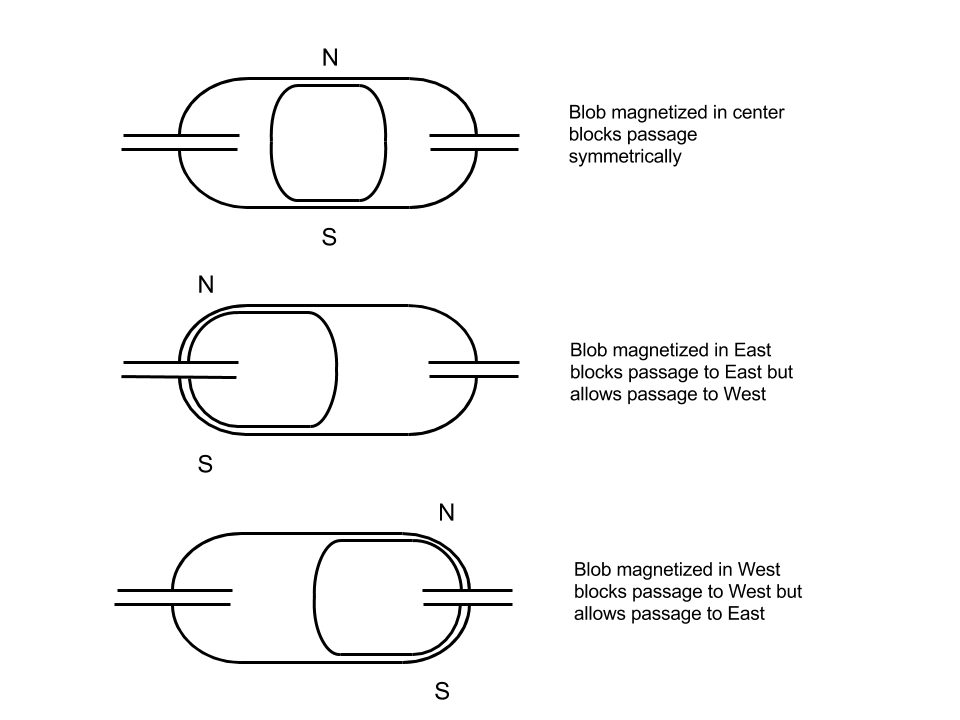
\includegraphics[width=1.0\textwidth]{BasicOperation.png}
     \caption{Basic Operation}
  \label{fig:closeup}     
\end{figure}


\section{Contact and Getting Involved}

Public Invention,
a free-libre, open-source research, hardware, and software project that welcomes volunteers.
To assist, contact:
\href{mailto:read.robert@gmail.com}{read.robert@gmail.com}.

\bibliographystyle{asmems4}
\bibliography{IEEEabrv,gluss}

\end{document}

https://infoscience.epfl.ch/record/55930/files/98.pdf

http://iris.elf.stuba.sk/jeeec/data/pdf/7s_110-41.pdf


